\documentclass[12pt]{article}

\usepackage{fancyhdr}
\usepackage{geometry}
\usepackage{ucs}
\usepackage[utf8x]{inputenc}
\usepackage[T1]{fontenc}
\usepackage[ngerman]{babel}
\usepackage{amsmath,amssymb,amstext}
\usepackage{hyperref}
\usepackage{cancel}
\usepackage{dsfont}
\usepackage{physics}
\usepackage{lmodern}
\usepackage{enumerate}
\usepackage{enumitem}
\usepackage{graphicx}
\usepackage{listings, color}
\usepackage[labelfont=bf]{caption}
\usepackage{titling}

\lstset{basicstyle=\scriptsize} %Quellcode mit Umlauten und ganz klein
\lstset{literate=
  {Ö}{{\"O}}1
  {Ä}{{\"A}}1
  {Ü}{{\"U}}1
  {ß}{{\ss}}2
  {ü}{{\"u}}1
  {ä}{{\"a}}1
  {ö}{{\"o}}1
}


%Geometrie----------------------------------------------------------------------------------------------------------

\geometry{a4paper, top=25mm, left=15mm, right=15mm, bottom=25mm,headsep=10mm, footskip=10mm}
\pagestyle{fancy}
\setlength{\parindent}{0pt} %Zeileneinrückung

\fancyhf{} %Setzt voreingestellte Kopf-und Fußzeilen-Eigenschaften zurück

\lhead{\nouppercase{\leftmark}}
\chead{}
\rhead{\thepage}

\lfoot{}
\cfoot{}
\rfoot{}

\title{\vspace{0cm}{\Huge Fortgeschrittenen-Praktikum I:\\ \vspace{1cm} Ultraschall}}
\author{Saskia Bondza\\Simon Stephan}
\date{durchgeführt am 20./21.09.2016}

\pretitle{%
  \begin{center}
  \LARGE
  
\includegraphics[width=6cm,]{figures/siegel}\\[\bigskipamount]
}
\posttitle{\end{center}}

%neue Commands----------------------------------------------------------------------------------------------------------
\newcommand{\nab}{\vec{\nabla}} %direkter Befehl mit Vektorpfeil
\newcommand{\gra}[3][0.7]{
	\begin{minipage}[h!]{\textwidth}
		\centering
		\includegraphics[width=#1\textwidth]{figures/#2.png}
		\captionof{figure}{#3}
	\end{minipage}
	\vskip 30 pt
}
\newcommand{\graTwo}[4][0.5]{
	\begin{minipage}[h!]{\textwidth}
		\centering
		\includegraphics[width=#1\textwidth]{figures/#2.png}
		\includegraphics[width=#1\textwidth]{figures/#3.png}
		\captionof{figure}{#4}
	\end{minipage}
	\vskip 30 pt
}
\newcommand{\del}[2][]{\frac{\partial #1}{\partial #2}}
\newcommand{\code}[1]{\texttt{#1}}


%Titel,Inhalt----------------------------------------------------------------------------------------------------------

\begin{document}
\pagenumbering{gobble} %verstecke Seitenzahl
\maketitle
\newpage

\thispagestyle{empty}
\section*{Abstract}


Im Rahmen dieses Versuches werden Grundlagen der Beugung an Amplituden- und Phasengittern und der Fourieroptik vermittelt. 
Hierzu werden die Gitterkonstanten eines Sinusgitters sowie verschiedener Amplitudengitter an Hand der Beugungsmaxima bestimmt. Zudem werden für die Amplitudengitter das Auflösungsvermögen und für eines dieser Gitter die Aperaturfunktion und Verhältnis der Spaltbreite zur Gitterkonstante bestimmt. 
Die wesentlichen Teile des Versuchsaufbaus, der verwendet wird, sind dabei eine monochromatischen, kohärenten Lichtquelle (ein Helium-Neon-Laser), die nach Durchgang durch eine Blende auf das Gitter (bzw. Ultraschallzelle) trifft, ein rotierender Motorspiegel der das zeitliche Signal in ein räunliches umwandelt, sowie an ein Oszilloskop angeschlossene Photodioden. Außerdem werden verschiedene Linsen und Spiegel verwendet um den Strahlengang geeignet zu lenken.
Unsere Ergebnisse...
\newpage
\tableofcontents
\newpage

%Schreiben----------------------------------------------------------------------------------------------------------
\pagenumbering{arabic} %verstecke Seitenzahl
\section{Einleitung}




\newpage
\section{Theoretische Grundlagen}
\newpage
\section{Sinusgitter}

\newpage
\subsection{Versuchsaufbau und -Durchführung}





\newpage
\subsection{Auswertung}

Aus den gemessenen Koordinaten der Punkte $P(x/y)$ der Maxima (siehe \ref{Laborheft})berechnen wir zunächst die Abstände $l_1 = \sqrt{x_1²+y_1²}$ und $l_2= \sqrt{x_2²+y_2²} $ zwischen dem Maximum $0.$ Ordnung und den Maxima $1.$ Ordnung. Aus den beiden Abständen zum linken und rechten Maximum $1.$ Ordnung berechnen wir einen gemittelten Abstand $l_{ges}$. Die Fehler berechnen wir mit Gauß'scher Fehlerfortpflanzung aus dem Fehler $s_{x/y}$ auf die Koordinaten:

\begin{align*}
s_{l_1} = s_{l_2} &= \sqrt{\left(\del[l]{x}\cdot s_{x/y}\right)^2+\left(\del[l]{y}\cdot s_{x/y}\right)^2}\\
&= s_{x/y}\\
\  \\
s_{l_{ges}} &= s_{x/y}/\sqrt{2}
\end{align*}

Wir erhalten:

 \vskip 10 pt
 \begin{table}[h!]
 {\centering{}
\begin{tabular}{c||c|c|c}
 					& $l_1$/cm 	& $l_2$/cm & $l{ges}$/cm	\\ \hline\hline
Messung 1		& $3.9 \pm 0.1$ 	&  $3.9 \pm 0.1$    	&  $3.95 \pm 0.07$ \\ \hline 
Messung 2	&	 $1.9 \pm 0.1$ 	   	&  $1.8 \pm 0.1$  	&  $1.87 \pm 0.07$  \\ \hline
Messung 3      	&  $5.0 \pm 0.1$  	&  $4.9 \pm 0.1$  &  $5.00 \pm 0.07$  \\ \hline
Messung 4    & $2.8 \pm 0.1$ & $2.9 \pm 0.1$ &   $2.88 \pm 0.07$        \\ \hline                                           
Messung 5  & $5.6 \pm 0.1$  & $5.7 \pm 0.1$ & $5.61 \pm 0.07$
 \end{tabular}}
 \caption{Abstände der Beugungsmaxima}
\end{table}
\vskip 10 pt

Hieraus lässt sich nun mit ref!!!!!! die Gitterkonstante berechnen wobei sich der Fehler wieder mit Gauß'scher Fehlerfortpflanzung berechnen lässt:

\begin{align*}
s_g = \sqrt{\left(\del[g]{l}\cdot s_{l}\right)^2+\left(\del[g]{d}\cdot s_{d}\right)^2}
\end{align*}

Wir erhalten:

\begin{itemize}
\item Messung 1: $g = 996 \pm 16$ nm
\item Messung 2: $g = 1082 \pm 40$ nm
\item Messung 3: $g = 989 \pm 13$ nm
\item Messung 4: $g = 994 \pm 23$ nm
\item Messung 5: $g = 995 \pm 12$ nm
\end{itemize}

Als Endergebnis berechnen wir nun noch das gewichtete Mittel mit Fehler:

\begin{align*}
g_{ges} &=\frac{\sum\limits_i \frac{1}{\sigma_i²} \cdot g_i}{\sum\limits_i \frac{1}{\sigma_i²}}\\
s_{g_{ges}} &= \frac{1}{\sum\limits_i \frac{1}{\sigma_i²}}
\end{align*}

und erhalten:

\begin{align*}
g_{ges} = 996 \pm 7 nm
\end{align*}

\newpage
\subsection{Diskussion}

\newpage
\section{Amplitudengitter}

\newpage
\subsection{Versuchsaufbau und -Durchführung}





\newpage
\subsection{Auswertung}

\subsubsection{Aperturfunktion}


Wir bestimmen die Aperturfunktion für Gitter 1, da wir hier die meisten Maxima beobachten konnten (siehe Abbildung ref!!!).
Aus den Amplituden der gefitteten  Gaußfunktionen erhalten wir hierbei die Intensität, wobei wir wir für jedes Maximum die Amplitude aus linkem und rechtem Maximum gewichtet mitteln (siehe ref!!!). 
 \vskip 10 pt
 \begin{table}[h!]
 {\centering{}
\begin{tabular}{c||c|c|c}
 					& $I_1/V$ 	& $I_2/V$ & $I_{ges}/V$	\\ \hline\hline
Maximum 5. Ordnung     & $0.08 \pm 0.14$  & $0.040 \pm 0.009$      &  $0.04012 \pm  0.00008$                       \\ \hline
Maximum 4. Ordnung		& $0.186 \pm 0.009$ 	&  $0.177 \pm 0.009$    	&  $0.182 \pm 0.006$ \\ \hline 
Maximum 3. Ordnung	&	 $0.402 \pm 0.009$ 	   	&  $0.447 \pm 0.010$  	&  $0.425 \pm 0.007$  \\ \hline
Maximum 2. Ordnung      	&  $0.95 \pm 0.02$  	&  $0.92 \pm 0.02$  &  $0.935 \pm 0.014$  \\ \hline
Maximum 1. Ordnung    & $2.8 \pm 0.1$ & $2.9 \pm 0.1$ &   $2.88 \pm 0.07$        \\ \hline                                           
Maximumg 0. Ordnung  & -  & - & $2.72 \pm 0.06$
 \end{tabular}}
 \caption{Abstände der Beugungsmaxima}
\end{table}
\vskip 10 pt


Aus diesen und der zuvor berechneten Gitterkonstante $g_1 =    $ (siehe ref!!!) läaat sich mittels der Fourierreihe (siehe ref!!!) nun die Aperturfunktion näherungsweise bestimmen:

FORMEL







\newpage
\subsection{Diskussion\label{BOOOOOMMMM!!!!!!!!!}} 

\section{Ultraschall-Phasengitter}

\newpage
\subsection{Versuchsaufbau und -Durchführung}





\newpage
\subsection{Auswertung}


\newpage
\subsection{Diskussion}

\newpage
\section{Zusammenfassung und Diskussion}

\subsection{Zusammenfassung der Ergebnisse}



\subsection{Diskussion}


\newpage
\section{Anhang} 


\subsection{Laborheft\label{Laborheft}} 
\begin{minipage}{\textwidth}
\centering
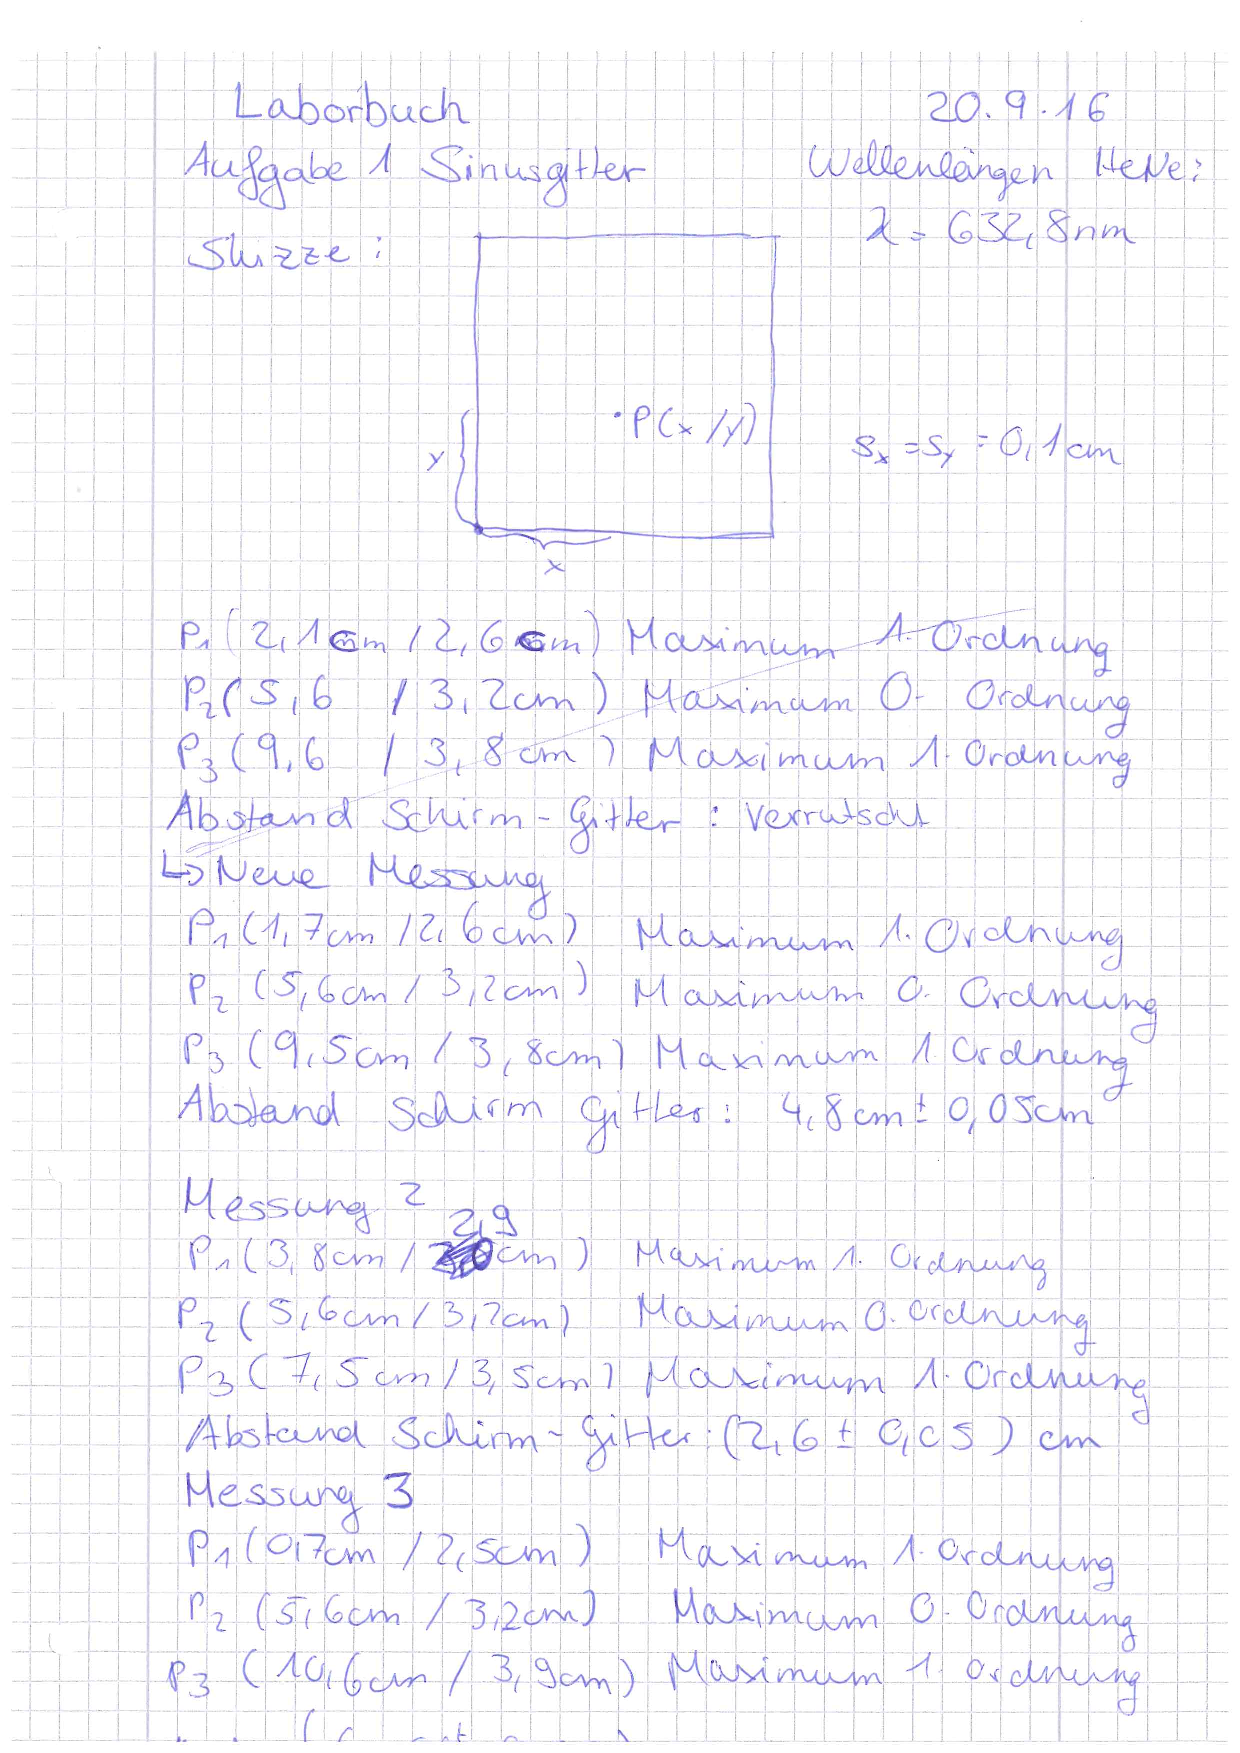
\includegraphics[width=0.9\textwidth]{figures/Laborbuch2.pdf}
\end{minipage}

\begin{minipage}{\textwidth}
\centering
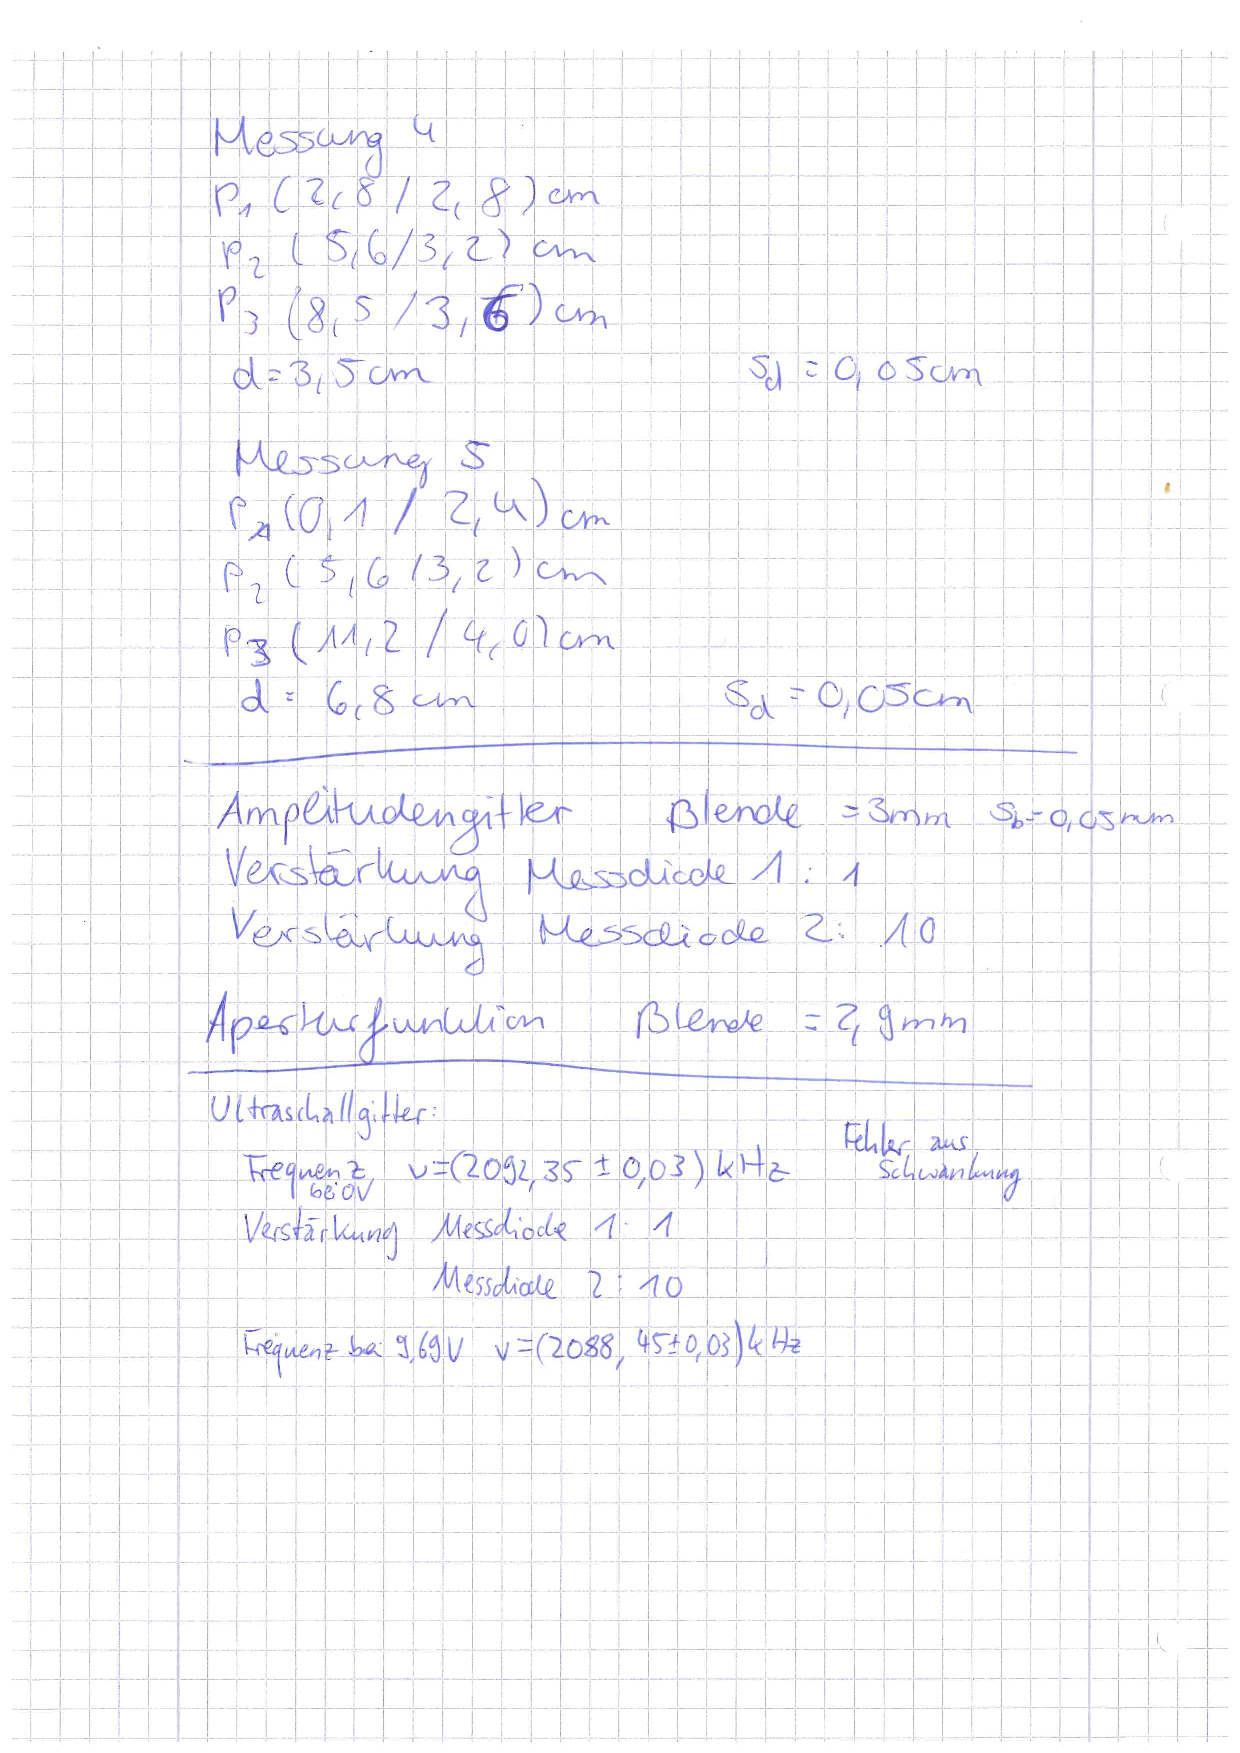
\includegraphics[width=0.9\textwidth]{figures/Laborbuch1.pdf}
\end{minipage}
\newpage
\listoffigures

%Literatur----------------------------------------------------------------------------------------------------------

%\cite{les}
\newpage
\thispagestyle{empty}
\begin{thebibliography}{9}

%\bibitem{staat}
%  Tobijas Kotyk,
%  \emph{Versuche zur Radioaktivität im Physikalischen Fortgeschrittenen Praktikum an der Albert-Ludwigs-Universität Freiburg},
%  Albert-Ludwigs-Universität, Freiburg,
%  2005
  

  
%\bibitem{molmasse}
%  \emph{http://www.convertunits.com/molarmass/<ELEMENTNAME AUF ENGLISCH>}, Stand 28.09.2015
  
\bibitem{bibhall}
\emph{http://www.schule-bw.de/unterricht/faecher/physik/online\_material/e\_lehre\_2/teilchenfeld/\\halleffekt.htm}, Stand 15.09.2016

\bibitem{anleitung}
\emph{http://hacol13.physik.uni-freiburg.de/fp/Versuche/FP1/FP1-8-Kernspinresonanz/Anleitung.pdf}, Stand 15.09.2016

\bibitem{Babykatze}
\emph{http://hacol13.physik.uni-freiburg.de/fp/Versuche/FP1/FP1-8-Kernspinresonanz/Anhang/A.Klett.pdf}, Stand 19.09.2016
\end{thebibliography}

\end{document}